% EF2039 PA04 paper, based on the CVPR 2026 template (https://github.com/cvpr-org/author-kit).
% Build: upload this folder to Overleaf as a zip, or run `latexmk -pdf main.tex`.

\documentclass[10pt,twocolumn,letterpaper]{article}

\usepackage[pagenumbers]{cvpr}

%% This file contains a number of tweaks that are typically applied to the main document.
%% They are not enabled by default, but can be enabled by uncommenting the relevant lines.

%%
%% Inline annotations; for predefined colors, refer to "dvipsnames" in the xcolor package:
%% https://tinyurl.com/overleaf-colors
%%
\newcommand{\red}[1]{{\color{red}#1}}
\newcommand{\todo}[1]{{\color{red}#1}}
\newcommand{\TODO}[1]{\textbf{\color{red}[TODO: #1]}}
%%
%% disable for camera ready / submission by uncommenting these lines  
%%
% \renewcommand{\TODO}[1]{}
% \renewcommand{\todo}[1]{#1}

%%
%% work harder in optimizing text layout. Typically shrinks text by 1/6 of page, enable
%% it at the very end of the writing process, when you are just above the page limit
%%
% \usepackage{microtype}

%%
%% fine-tune paragraph spacing
%%
% \renewcommand{\paragraph}[1]{\vspace{.5em}\noindent\textbf{#1.}}

%%
%% globally adjusts space between figure and caption
%%
% \setlength{\abovecaptionskip}{.5em}


%%
%% Allows "the use of \paper to refer to the project name"
%% with automatic management of space at the end of the word
%%
% \usepackage{xspace}
% \newcommand{\paper}{ProjectName\xspace}

%%
%% Commonly used math definitions
%%
% \DeclareMathOperator*{\argmin}{arg\,min}
% \DeclareMathOperator*{\argmax}{arg\,max}

%%
%% Tigthen underline
%%
% \usepackage{soul}
% \setuldepth{foobar}
\usepackage{booktabs}

\definecolor{cvprblue}{rgb}{0.21,0.49,0.74}
\usepackage[pagebackref,breaklinks,colorlinks,allcolors=cvprblue]{hyperref}

\def\paperID{PA04}
\def\confName{EF2039}
\def\confYear{2026}

\newcommand{\repo}{\url{https://github.com/InKang-1028/AI_programing}}

\title{How Training Data Shapes an Image Classifier:\\Class Imbalance and Label Noise in Teachable Machine}

\author{Inkang Jeong (20250631)\\
School of Energy Engineering, KENTECH\\
{\tt\small wjddlsrkd@kentech.ac.kr}
}

\begin{document}
\maketitle
\begin{abstract}
Real training data is rarely balanced or perfectly labeled.
We ask how much two such flaws, class imbalance and label noise, hurt a 5-class flower classifier built with
Teachable Machine.
From a balanced set of 200 TF Flowers images per class, we train seven models that each change one property of
the data, and test them all on the same 500 held-out images.
When roses is cut from 200 to 5 training images, its accuracy falls from 84\% to 2\%, while the other classes stay at
82--93\%; most of the missing roses are predicted as tulips.
When 10, 30, and 50\% of the labels are flipped, accuracy falls from 86.6\% to 81.6, 72.0, and 54.2\%, and every
class loses about equally.
Imbalance thus damages one class while overall accuracy hides it; noise damages all classes.
\end{abstract}

\begin{figure*}[t]
  \centering
  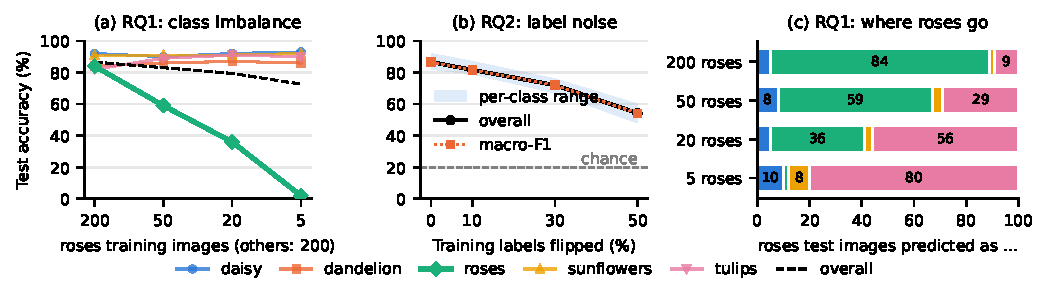
\includegraphics[width=\linewidth]{figures/fig_paper.pdf}
  \vspace{-1.8em}
  \caption{\textbf{(a)} RQ1: per-class test accuracy as roses training images decrease; only roses collapses.
  \textbf{(b)} RQ2: accuracy and macro-F1 (almost identical) as more training labels are flipped.
  The shaded band spans the five per-class accuracies.
  \textbf{(c)} How each RQ1 model classifies the 100 roses test images. The missing roses go mostly to tulips.}
  \label{fig:main}
  \vspace{-0.8em}
\end{figure*}

\section{Introduction}
\label{sec:intro}

A classifier can only learn what its training data shows it.
In practice, that data is often small, dominated by a few common classes, and sprinkled with labeling
mistakes~\cite{buda2018imbalance,song2022noisy}.
Teachable Machine (TM)~\cite{carney2020tm} lets anyone train an image classifier from a few hundred images,
so it is worth knowing how it copes when those images are not ideal.
We study two data-related research questions:

\noindent\textbf{RQ1 (class imbalance).} When one class has far fewer training images than the others,
what happens to its accuracy, and to the accuracy of the other classes?

\noindent\textbf{RQ2 (label noise).} When part of the training labels is wrong, how much does accuracy drop,
and is the drop shared evenly across classes?

\section{Method}
\label{sec:method}

\paragraph{Data.}
We use TF Flowers~\cite{tfflowers}, which contains 3,670 Flickr photos of five flower types
(633--898 per class, CC BY 2.0).
With random seed 0 (Python \texttt{random}), we set aside a balanced \textbf{test set of 100 images per class},
never used for training, and draw a balanced \texttt{base} training set of 200 images per class from the rest;
every other training set changes exactly one property of it (\cref{tab:results}).
For RQ1, only roses is reduced to 50, 20, or 5 images, and each smaller set is a subset of the larger one.
For RQ2, the first 10, 30, or 50\% of each class (in the seed-0 order) are relabeled as the other four classes in
equal shares; every class keeps 200 images, so only the labels change.
The file list of every split is released as CSV.

\paragraph{Model and training.}
All models are trained in TM's image project with its default settings: 50 epochs, batch size 16, and learning
rate 0.001.
TM keeps a pretrained MobileNetV2~\cite{sandler2018mobilenetv2} (width 0.35, 224$\times$224 input) frozen and
trains only a small head (Dense 100, ReLU, 5-way softmax) with Adam~\cite{kingma2015adam}.
It holds out a random 15\% of the uploaded images for its own validation, so about 170 images per class are
actually used for training.
Models were trained on Nov.~15, 2026 in the TM web app (one new project each) and exported as Keras \texttt{.h5}.

\paragraph{Evaluation.}
Test images are preprocessed the same way as in TM's export: RGB, center crop, resize to 224$\times$224,
and scale to $[-1,1]$.
We report per-class accuracy (recall), overall accuracy, macro-F1, and confusion matrices.
TM's internal validation scores are not used: they rest on 1--30 images per class and, under noise, on noisy labels.
Evaluation uses Python 3.10 and TensorFlow 2.15.1; evaluating all seven models takes about 36\,s on CPU.

\section{Experiments}
\label{sec:experiments}

\begin{table}[t]
\centering\footnotesize
\setlength{\tabcolsep}{1.7pt}
\begin{tabular}{lcc|ccccc|cc}
\toprule
& \multicolumn{2}{c|}{Training set} & \multicolumn{5}{c|}{Per-class accuracy} & & \\
Model & \#Ros. & Noise & Dai. & Dan. & Ros. & Sun. & Tul. & Acc. & F1 \\
\midrule
base & 200 & 0 & 92 & 84 & 84 & 91 & 82 & 86.6 & 86.6 \\
\midrule
imb\_roses50 & 50 & 0 & 90 & 86 & 59 & 91 & 89 & 83.0 & 82.7 \\
imb\_roses20 & 20 & 0 & 92 & 87 & 36 & 91 & 91 & 79.4 & 78.3 \\
imb\_roses5 & 5 & 0 & 93 & 86 & \textbf{2} & 92 & 90 & 72.6 & 66.5 \\
\midrule
noise10 & 200 & 10 & 83 & 79 & 80 & 87 & 79 & 81.6 & 81.6 \\
noise30 & 200 & 30 & 75 & 72 & 70 & 76 & 67 & 72.0 & 72.0 \\
noise50 & 200 & 50 & 54 & 53 & 56 & 60 & 48 & 54.2 & 54.2 \\
\bottomrule
\end{tabular}
\caption{Training sets and test results (\%). \#Ros.: roses training images (others: 200); Noise: \% of training labels flipped. Per-class accuracy is recall; F1 is macro-F1.}
\label{tab:results}
\end{table}


The balanced \texttt{base} model reaches 86.6\%; its most common mistake is confusing roses and tulips
(9 images each way), which share red and pink petals.

\paragraph{RQ1: class imbalance.}
As roses training images drop from 200 to 50, 20, and 5, roses accuracy falls from 84\% to 59, 36, and 2\%.
Even a 4:1 imbalance costs 25 points.
The other four classes, in contrast, hardly change (82--93\%), and tulips actually improves from 82 to 90\%.
\Cref{fig:main}c explains why: the roses the model no longer recognizes are mostly labeled as tulips
(9, 29, 56, and 80 of 100), the class they already resembled.
With only 5 roses, the model predicts tulips 184 times for 100 real tulips, so tulip precision drops to 49\%.
Overall accuracy (72.6\%) understates this failure, since roses is only 20\% of the test set;
macro-F1 (66.5\%) reveals it more clearly.

\paragraph{RQ2: label noise.}
With 10, 30, and 50\% of the labels flipped, accuracy falls from 86.6\% to 81.6, 72.0, and 54.2\%:
about 0.5 points per 1\% of noise up to 30\%, then 0.9 points per 1\% beyond it.
Unlike imbalance, noise hurts all classes about equally: the per-class band in \cref{fig:main}b stays narrow,
and macro-F1 stays within 0.1 points of accuracy.
The extra errors still fall mostly between similar classes; tulips predicted as roses rise from 9 to 18 and 23
at 0, 30, and 50\% noise.
Even at 50\% noise, the correct label remains the most common one in each class (50\% versus 12.5\% for each
wrong class), which keeps the model well above chance (20\%).

\paragraph{Comparison and limitations.}
Flipping 100 labels (\texttt{noise10}) costs 5.0 points across all classes, whereas removing 150 roses
(\texttt{imb\_roses50}) costs 3.6 points overall but 25 on roses.
Each model was trained once, and with 100 test images per class the 95\% interval is about $\pm$7 points per class
($\pm$3 overall), so small gaps such as tulips rising from 82 to 90\% are only suggestive.
We also tested a single minority class and symmetric synthetic noise, whereas real label errors tend to cluster
between similar classes.

\section{Conclusion}
\label{sec:conclusion}

Even with a strong pretrained backbone, class imbalance quietly gives the minority class away to its most similar neighbor,
so per-class accuracy or macro-F1 should be reported alongside overall accuracy.
Label noise instead lowers accuracy for every class, and the loss steepens beyond 30\% noise.
All code, data splits, trained models, TM project files, and step-by-step instructions are available at \repo.

{
    \small
    \bibliographystyle{ieeenat_fullname}
    \bibliography{main}
}

\end{document}
